\section{Auswertung}


\subsection{Gamma-Strahlung}
Die bei der Untersuchung der $\gamma$-Strahlung gemessene Nullrate $N_0$ bzw. die gemessene Aktivität $A_0$ ergaben bei einer Messdauer von $t = \SI{900}{s}$
\begin{equation}
    N_0 = 10005 \pm 32 \qquad \text{bzw.} \qquad A_0 = \SI{1.117 \pm 0.035}{\frac{1}{s}}. \notag
\end{equation}

Dabei wird bei der Zählrate von einem Fehler von $\Delta N = \sqrt{N}$ ausgegangen und über die Gaussche Fehlerfortpflanzung auch der Fehler für die Aktivität nach 
\begin{equation}
  \label{eq:fehler}
  \Del{A} = \frac{1}{t} \cdot \sqrt{N}
\end{equation} bestimmt.
Die Nullaktivität wird von den von den Messungen jeweils abgezogen.
Als Strahler wird \textsuperscript{137}Cs verwendet.

\subsubsection{Absorption von Zink}
Zunächst wird der Absorptionskoeffizient $\mu_\text{Zn}$ von Zink bestimmt.
Dazu werden die Aktivität und die Schichtdicke aus Tabelle \ref{tab:Zink} in einem halblogarithmischen Diagramm gegeneinander aufgetragen.

\begin{table}[H]
  \begin{center}
    \caption{Messung der Aktivitäten eines $\gamma$-Strahlers für eine Zinkabschrimung.}
    \label{tab:Zink}
    \begin{tabular}{c|c|c|c} 
      \textbf{Dicke $D$ $[cm]$} & \textbf{Messdauer $t$ $[s]$} & \textbf{Zählrate $N$} & \textbf{Aktivität $A$ - $A_0$ $[\frac{1}{s}]$}\\
      \hline
        0.21 & 40 & 4942 $\pm$ 70.30 & 123.55 $\pm$ 1.78 \\
        0.42 & 70 & 8476 $\pm$ 92.07 & 121.09 $\pm$ 1.32 \\
        0.63 & 90 & 9243 $\pm$ 96.14 & 102.70 $\pm$ 1.07 \\
        0.84 & 100 & 9133 $\pm$ 95.57 & 91.33 $\pm$ 0.96 \\
        1.05 & 110 & 9156 $\pm$ 95.69 & 83.24 $\pm$ 0.87 \\
        1.26 & 120 & 8828 $\pm$ 93.96 & 73.57 $\pm$ 0.78 \\
        1.47 & 130 & 9192 $\pm$ 95.88 & 70.71 $\pm$ 0.74 \\
        1.68 & 140 & 8855 $\pm$ 94.10 & 63.25 $\pm$ 0.67 \\
        1.89 & 150 & 8606 $\pm$ 92.77 & 57.37 $\pm$ 0.62 \\
        2.10 & 160 & 8443 $\pm$ 91.89 & 52.77 $\pm$ 0.57
    \end{tabular}
  \end{center}
\end{table}

Die Messwerte sind in der Abbildung \ref{fig:zink} dargestellt.
\begin{figure}[h]
  \centering
  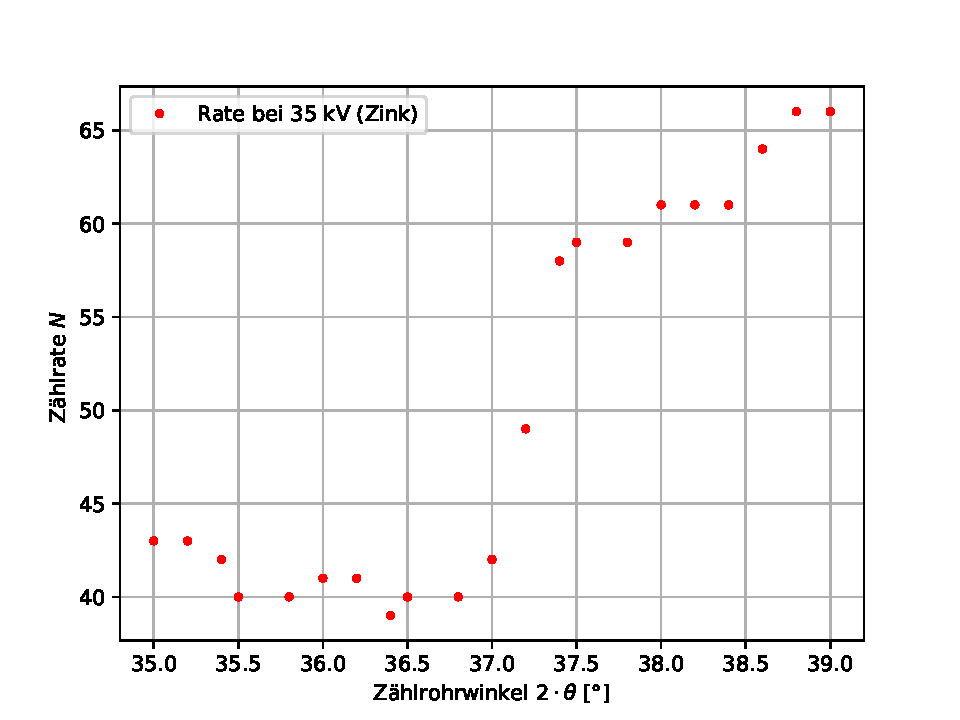
\includegraphics[height=8cm]{Auswertung/Zink.pdf}
  \caption{Aktivität gegen die Schichtdicke von Zink zur Bestimmung des Absorptionskoeffizienten aufgetragen.}
  \label{fig:zink}
\end{figure}

Mittels linearer Regression nach
\begin{equation}
  \label{eq:lin}
  y = - A \;x + B
\end{equation}
werden die beiden Parameter auf 
\begin{equation}
  A = \SI{0.474 \pm 0.019}{\frac{1}{cm}} \qquad \text{und} \qquad B = \SI{4.923 \pm 0.024}{\text{ln}\left (\frac{1}{s}\right)}
\end{equation}
bestimmt.
Die Anfangsaktivität $A(0)$ lässt sich durch exponieren von $B$ bestimmen.
Der Absoprtionskoeffizient lässt sich nach Umformung der Gleichung (3) und Berücksichtigung von Gleichung (4) als Steigung der Geraden
\begin{equation}
  \text{ln}(A) = \text{ln}(A(0)) - \mu \cdot d
\end{equation}
bestimmen.
Dabei ergeben sich der Absoprtionskoeffizient von Zink und die Anfangsaktivität
\begin{equation}
  \mu_\text{Zink} = A = \SI{47.4 \pm 1.9}{\frac{1}{m}} \qquad \text{und} \qquad A(0) = \text{exp}(B) = \SI{137.414 \pm 1.025}{\frac{1}{s}}.   \notag
\end{equation}
Zusätzlich wird der theoretische Wert für den Compton-Absorptionskoeffizienten nach Gleichung (5) und (6) berechnet.
Über das angenommene Verhältnis von \textsuperscript{137}Cs-Strahlung
\begin{equation}
  \epsilon = \frac{E_\text{$\gamma$}}{m_0c^2} = 1,295
\end{equation}
wird der theoretische Wert auf
\begin{equation}
    \mu_\text{Comp,Zink} = \SI{50,380}{\frac{1}{m}}
\end{equation}
bestimmt.

\subsubsection{Absorption von Blei}
Analog dazu wird der Absorptionskoeffizient von Blei untersucht.
Die in Tabelle \ref{tab:Blei} aufgelisteten Werte werden in Abbildung \ref{fig:blei} halblogarithmisch gegeneinander aufgetragen.
Es wird wie bei der Zinkabschrimung der Strahler \textsuperscript{137}Cs verwendet.

\begin{table}[H]
  \begin{center}
    \caption{Messung der Aktivitäten eines $\gamma$-Strahlers für eine Bleiabschrimung.}
    \label{tab:Blei}
    \begin{tabular}{c|c|c|c} 
      \textbf{Dicke $D$ $[cm]$} & \textbf{Messdauer $t$ $[s]$} & \textbf{Zählrate $N$} & \textbf{Aktivität $A - A_0$ $[\frac{1}{s}]$}\\
      \hline
        0.1 & 40 & 5173 $\pm$ 72 & 129.33 $\pm$ 1.80 \\
        0.2 & 60 & 6682 $\pm$ 82 & 111.37 $\pm$ 1.36 \\
        0.3 & 70 & 7289 $\pm$ 85 & 104.13 $\pm$ 1.22 \\
        0.6 & 80 & 5374 $\pm$ 74 & 67.18 $\pm$ 0.92 \\
        1.03 & 90 & 4088 $\pm$ 63 & 45.42 $\pm$ 0.71 \\
        1.33 & 100 & 3336 $\pm$ 58 & 33.36 $\pm$ 0.58 \\
        2.06 & 130 & 1968 $\pm$ 45 & 15.14 $\pm$ 0.34 \\
        3.05 & 200 & 1427 $\pm$ 37 & 7.14 $\pm$ 0.19 \\
        4.04 & 350 & 1144 $\pm$ 34 & 3.27 $\pm$ 0.10 \\
        5.07 & 500 & 940 $\pm$ 31 & 1.88 $\pm$ 0.06
    \end{tabular}
  \end{center}
\end{table}

\begin{figure}[h]
  \centering
  \includegraphics[height=8cm]{Auswertung/Blei.pdf}
  \caption{Aktivität gegen die Schichtdicke von Blei zur Bestimmung des Absorptionskoeffizienten aufgetragen.}
  \label{fig:blei}
\end{figure}

Die lineare Regression nach Gleichung \ref{eq:lin} liefert die Parameter
\begin{equation}
  A = \SI{1.021 \pm 0.016}{\frac{1}{cm}} \qquad \text{und} \qquad B = \SI{4.870 \pm 0.043}{\text{ln}\left (\frac{1}{s}\right)}. \notag
\end{equation}
Daraus ergeben sich analog zur Bestimmung des Absoprtionskoeffizienten und der Anfangsaktivität
\begin{equation}
  \mu_\text{Blei} = \SI{102.1 \pm 1.6}{\frac{1}{m}} \qquad \text{und} \qquad A(0) = \SI{130.321 \pm 1.039}{\frac{1}{s}}.  \notag 
\end{equation}

Der theoretische Wert für den Compton-Absorptionskoeffizienten von Blei beträgt nach Gleichung (5) und (6)
\begin{equation}
  \mu_\text{Comp,Blei} = \SI{69.229}{\frac{1}{m}}. \notag
\end{equation}

\subsection{Beta-Strahlung}
Die bei der Untersuchung der $\beta$-Strahlung gemessene Nullrate $N_0$ bzw. die gemessene Aktivität $A_0$ ergaben bei einer Messdauer von $t = \SI{900}{s}$
\begin{equation}
    N_0 = 598 \pm 24 \qquad \text{bzw.} \qquad A_0 = \SI{0.664 \pm 0.027}{\frac{1}{s}}. \notag
\end{equation}
Dabei beträgt der Fehler der Zählrate $\Delta N = \sqrt{N}$ und der daraus resultierende Fehler für die Aktivität wird nach Gleichung \ref{eq:fehler} bestimmt.
Zur Bestimmung der maximalen Reichweite $r_\text{max}$ der $\beta$-Teilchen wird nun die Zählrate gegen die Massenbelegung $R$ in einem halblogarithmischen Diagramm aufgetragen.
Die Massenbelegung $R$ ergibt sich aus Gleichung (7) und der Dicht von Aluminium mit
\begin{equation}
  \rho_\text{Aluminium} = \SI{2698.9}{\frac{kg}{m^3}}. \notag
\end{equation}
Dabei werden wie in Abbildung \ref{fig:BetaVerlauf} erkennbar ist die beiden linearen Abschnitte oberhalb und unterhalb von $R_\text{max}$ untersucht.
$R_\text{max}$ ist dabei der entsprechende Wert der Massenbelegung für den maximalen Abstand $r_\text{max}$, den die $\beta$-Teilchen zurücklegen können.

\begin{table}[H]
  \begin{center}
    \caption{.}
    \label{tab:tres}
    \begin{tabular}{c|c|c|c} 
      \textbf{Dicke $D$ $[\mu m]$} & \textbf{Messdauer $t$ $[s]$} & \textbf{Impulse $N$} & \textbf{Zählrate $A - A_0$ $[\frac{1}{s}]$}\\
      \hline
      100 $\pm$ 0.0 & 100 & 4029 $\pm$ 63 & 39.62 $\pm$ 0.74\\
      125 $\pm$ 0.0 & 200 & 2016 $\pm$ 45 & 9.42 $\pm$ 0.22\\
      153 $\pm$ 0.5 & 300 & 2868 $\pm$ 54 & 8.89 $\pm$ 0.18\\
      160 $\pm$ 1.0 & 400 & 2334 $\pm$ 48 & 5.17 $\pm$ 0.12\\
      200 $\pm$ 1.0 & 500 & 1140 $\pm$ 34 & 1.61 $\pm$ 0.07\\
      253 $\pm$ 1.0 & 600 & 489 $\pm$ 22 & 0.15 $\pm$ 0.04\\
      302 $\pm$ 1.0 & 700 & 533 $\pm$ 23 & 0.10 $\pm$ 0.03\\
      338 $\pm$ 5.0 & 800 & 529 $\pm$ 23 & 0.08 $\pm$ 0.03\\
      400 $\pm$ 1.0 & 900 & 659 $\pm$ 26 & 0.07 $\pm$ 0.03\\
      444 $\pm$ 2.0 & 1000 & 692 $\pm$ 26 & 0.03 $\pm$ 0.02
    \end{tabular}
  \end{center}
\end{table}

Über die lineare Regression der Form
\begin{equation}
  y = A_i \; x + B_i \;\;\;\; (i = 1,2)
\end{equation} werden nun die Parameter der beiden Geraden bestimmt.
Die Messwerte aus Tabelle \ref{tab:tres} und die Ausgleichgeraden sind in Abbildung \ref{fig:Beta} dargestellt.
\begin{figure}[h]
  \centering
  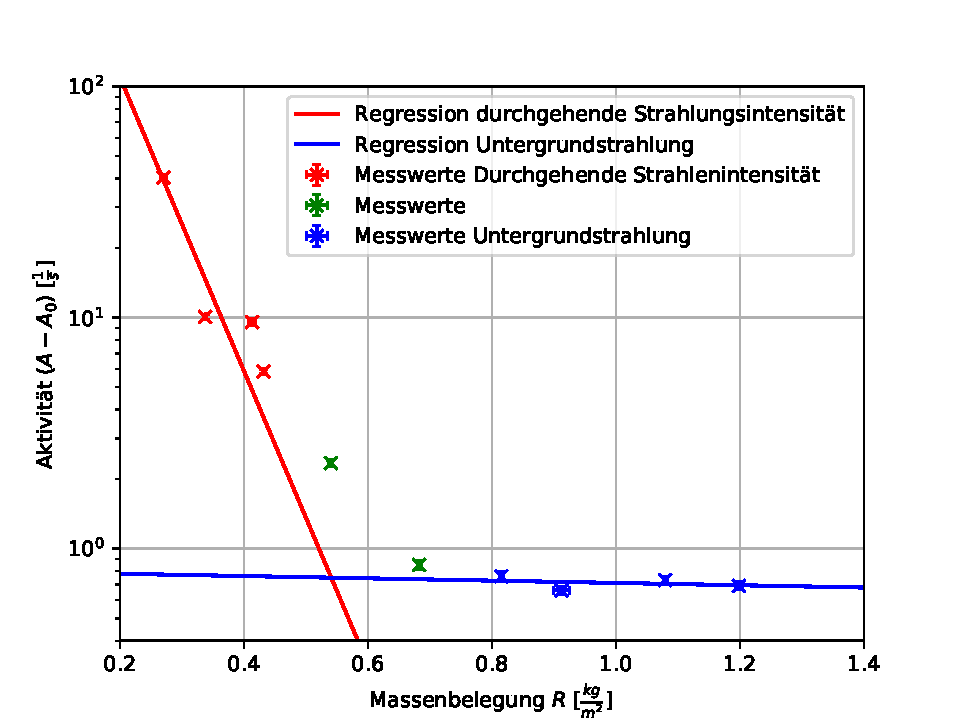
\includegraphics[height=8cm]{Auswertung/BetaKurve.pdf}
  \caption{Die beta-Absorptionskurve mit der durchgehenden Strahlungsintensität (rot) und der Untergrundstrahlung(blau).}
  \label{fig:Beta}
\end{figure}
Dabei werden zwei grün markierte Werte ausgelassen, da diese sich in der Nähe des nichtlinearen Gebietes um $R_\text{max}$ befinden und somit die lineare Regression verfälschen würden.
Des Weiteren folgen diese Werte nicht mehr der guten Näherung des Absorptionsgesetzes nach Gleichung (3), wodurch große Abweichungen autreten würden.
Außerdem folgen die Werte knapp um $R_\text{max}$ auch nicht der Untergrundstrahlung, die durch die Bremsstrahlung erfolgt.
Für das Gebiet der durchgehende Strahlungsintensität ergeben sich die Parameter
\begin{equation}
  A_1 = \SI{-14.622 \pm 15.249}{\frac{1/s}{kg/m^2}} \qquad \text{und} \qquad B_1 = \SI{7.612 \pm 1.218}{\frac{1}{s}} \notag
\end{equation}
Die Paramter der Untergrundstrahlung ergeben
\begin{equation}
  A_2 = \SI{-0.115 \pm 0.059}{\frac{1/s}{kg/m^2}} \qquad \text{und} \qquad B_2 = \SI{-0.226 \pm 0.060}{\frac{1}{s}}.  \notag
\end{equation}

Die Stelle des Schnittpunktes ergibt nun die maximale Reichweite der $\beta$-Teilchen als Massenbelegung mit
\begin{equation}
  R_\text{max} = \frac{B_2 - B_1}{A_2 -A_1}.
\end{equation}
Der dazugehörige Fehler nach Gau\ss{} ergibt sich nach der Gaußschen Fehlerfortpflanzung und der daraus berechnete Fehler mit
\begin{equation}
  \begin{split}
        \increment R_\text{max} &= \biggl(\left(\frac{1}{A_1 - A_2} \cdot \increment B_2\right)^2 + \left(-\frac{1}{A_1 - A_2} \cdot \increment B_1\right)^2 \\
         &+ \left(-\frac{B_2 - B_1}{(A_1 - A_2)^2} \cdot \increment A_1\right)^2 + \left(\frac{B_2 - B_1}{(A_1 - A_2)^2} \cdot \increment A_2\right)^2\biggr)^{\frac{1}{2}}.
  \end{split}
\end{equation}

Für die maximale Reichweite und deren Massenbelegung ergeben sich
\begin{equation}
  r_\text{max} = \SI{200 \pm 210}{\mu m}\qquad \text{und} \qquad R_\text{max} = \SI{0.541 \pm 0.575}{\frac{kg}{m^2}}.
\end{equation}
Damit lässt sich nun die maximale Energie der $\beta$-Strahlung nach Gleichung (8) auf
\begin{equation}
  E_\text{max} = \SI{0.234 \pm 0.149}{MeV}
\end{equation}
bestimmen.
